\documentclass[titlepage,10pt]{article}
\usepackage{textcomp}
\usepackage{latexsym}
\usepackage{graphicx}
\usepackage{amsmath}
\usepackage{moreverb} 
\usepackage{pdflscape}
%\usepackage[hmargin=3cm,vmargin=3.5cm]{geometry}


\def\urltilda{\kern -.15em\lower .7ex\hbox{\~{}}\kern .04em}


\begin{document}
\title{
Scaled SWIFT \\
Research Proposal
}

\author{Zouhair Mahboubi}

\date{March $1^{st}$, 2010\\ Stanford University}

\maketitle
\newpage

\abstract
This paper is meant to be a quick overview of the research potential of building a scaled SWIFT model. The goal of the research is to understand effects of scaling on the aerodynamic performance and dynamic response of sub-scale models. We hope to eventually establish a theory and framework to compensate for these effects, in order to be able to better predict in the future for which maneuvers the performance and dynamic parameters obtained from the sub-scale are representative of the full-scale. \\

In the paper, we motivate our choice of the SWIFT as a platform and highlight the potential of collaboration with NASA Ames. We then present some preliminary results of weight, power and price estimation as well as aerodynamic performance for 3 different scales (1/2, 1/3 and 1/4) 

\newpage
\section{Introduction}
The SWIFT is a foot-launched hang-glider with performance similar to a sailplane. The plane has been flown for many years and won numerous competitions. It has also been converted to a powered plane in a pusher-prop configuration. Recently, NASA Ames Research Center (ARC) purchased one of these planes and is planning on converting the airplane into an electrically powered Unmanned Aerial Vehicle (UAV) that would be capable of serving as a technology demonstrator.\\
Our goal is to develop one or two sub-scale models of the SWIFT which can be used as a platform for research in both controls and applied aerodynamics. We intend to coordinate our efforts with the on-going research on the full-scale aircraft, in the hope that data, algorithms, models, etc. can be shared and used on both vehicles.

\section{Motivation}
\subsection{the SWIFT as a platform}
Generally speaking, the weight of a scale-model is proportional to the cube of the scale. With a smaller weight and surface area, the drag of the model airplane and therefore the propulsive power requirement are significantly smaller. With the lower power requirements and reduced weight, a model plane is safer to operate, and cheaper to construct and maintain. Turn-around time for flight-tests is also quicker given the reduced complexity of flight-logistics: model aircrafts are regulated by the Academy of Model Aeronautics (AMA), whereas UAVs operating in the NAS must follow FAA guidelines and need to obtain a permit.\\

In the short term, a scale-model of the SWIFT could be used by NASA-ARC for testing planned modifications or new control algorithms before implementing them on the full-scale plane. This means the possibility of demonstrating new concepts quicker, safer and cheaper. \\

\enlargethispage{2\baselineskip}
The difficulty is in ensuring that the model will have performance and handling qualities similar to those of the full-scale. In order to do this, the scaling needs to maintain some similitude requirements \cite{Wolowicz} (non-dimensional coefficients describing the aerodynamics and dynamics need to be matched). However, it is usually difficult to have all of them matching. And although the use of scale-models for testing aircraft performance is not a new concept, it is still unclear how much error is introduced by incorrect scaling. For these reasons, the SWIFT is an attractive platform given that we would have access to flight-test data of both the model and scale airplanes, thus allowing us to quantify uncertainties on the estimates of performance and dynamic properties caused by unmatched similitude coefficients. Per example, it would be possible to find out which stability derivatives can be trusted from system identification when Reynolds numbers are not matched. We would then investigate methods to account for the discrepancies.\\

\subsection{Research Applications}
The main goal of this project is to establish a theory and framework which would lead to a better understanding of the effects of scaling on aerodynamic performance and dynamic response. In the process, we plan to come-up with methods that would account for these effects in order to better predict the performance of the full-scale model.\\

But since we will have at our disposal a UAV with a relatively high aerodynamic efficiency, we can use it as a testbed for other on-going projects within the Aircraft Design Group: per example dynamic soaring, or characterization of propeller noise (and how it scales). \\

The SWIFT has a low wing loading, and is likely to benefit from solar power. But it's unclear how the addition of panels to the wing affect the airfoil's performance (changing roughness, turbulence onset, etc.) and how the solar-power can be optimally integrated with battery power. This can be investigated on the sub-scale model, and alongside the other applications, could eventually benefit NASA's full-scale UAV. 

\subsection{Literature review}
As mentioned before, the use of models for testing aircraft concepts is not new. NASA itself has a history of using unmanned sub-scale models such as the X-38 Crew Return Vehicle, or the more recent X-48 Blended-Wing-Body demonstrator. But generally speaking, the trend is to construct a scaled model to demonstrate a new technology, before the full-scale airplane is built. One can imagine that at the prototype stage, much of the design is not yet frozen and the full-scale is likely to be different from the sub-scale, thus making it hard to compare flight-test results between the model and the full-scale.\\

A notable exception is NASA's AirSTAR program in which a 5.5\% dynamically scaled version of a B757 was built. The focus of the program however is on 'Integrated Resilient Aircraft Control' which would help prevent loss-of-control accidents. As mentioned in \cite{Airstar} "AirSTAR testbed will be used for [experiments] such as loss-of-control flight due to high angles-of-attack and sideslip, [where] the flow around the aircraft becomes separated and fluid effects associated with Reynolds number scaling may be minimized. For more benign flight conditions, Reynolds number effects can be significant and the aerodynamics of the model would not be representative of the full scale aircraft for certain maneuvers."\\

Our goal is different in that we want to actually understand how significant these effects can be, in order to be able to better predict in the future for which maneuvers the performance and dynamic parameters are representative.

\section{Methodology}
\subsection{Initial Sizing}
\label{sec:initialsizing}
We plan to use traditional methods for the construction (i.e. foam-core and balsa wood mostly) and rely on off-the-shelf RC hobbyist parts and materials to keep the cost down. Initial weight and price estimates (alongside some assumptions) are summarized in Table \ref{tab:scales} and figure \ref{fig:scales}.\\

Based on initial sizing, a 1/4 scale model would be straight-forward to construct and operate, a 1/3 scale-model would be useful while remaining manageable, while a 1/2 scale is doable with off-the-shelf RC hobbyist parts but the logistics for operation are somewhat harder. The assumptions and approach used to come up with weight, power and price estimates are outlined in appendix \ref{app:excel}. We leave the decision of which scale should be pursued to after the discussion about Reynold numbers. The details of the computation steps are given as comments in the spreadsheet.

\begin{table}[h]
\begin{center}
\begin{tabular}{|c|c|c|c|c|}
\hline
Scale $\lambda$	& 1 & 1/2 & 1/3 & 1/4 \\ \hline
Span (m)	& 13& 6.5 & 4.3 & 3.25\\ 
Mass (kg)	& 150& 14 & 5   & 3 \\
Cruise(m/s)	& 17 & 10 & 9   & 9.5 \\
$Re_{avg}$  	& 1,150,000 & 330,000 & 200,000 & 160,000 \\
Froude		& 29.5 & 20.6 & 25.0 & 36.6 \\
Motor Power (W) & 11000 & 1000 & 350 & 220 \\
Endurance (min) & 180  & 20 & 20 & 20 \\
Price (\$)      & $>$40000 & 5200 & 3800 & 3200 \\
\hline
\end{tabular}
\caption{Scale Comparison}
\label{tab:scales}
\end{center}
\end{table}

The price estimates for the models are for the material and components and include about \$2000 for the autopilot and sensors. Figure \ref{fig:scales} plots the ratios of these estimates relative to the full-scale airplane. These results which are obtained from individual component build-up seem to agree with the 'rule of thumb' that mass is roughly cubic in the scale $\lambda$. Price and power are strongly dependent on weight so it's no surprise that their trends are similar to the mass. We also notice that the Reynolds number varies with $\lambda^{1.5}$: this is expected since if the mass is cubic in scale and lift-coefficient is assumed to be constant, the velocity varies with $\sqrt{\lambda}$. The Froude number $Fr =\frac{V^2}{g \bar{c}}$ so it should be proportional to $\frac{{\sqrt{\lambda}}^2}{\lambda}=1$, which explains why the ratio is 'around' 1.

\begin{figure}[h]
\begin{center}
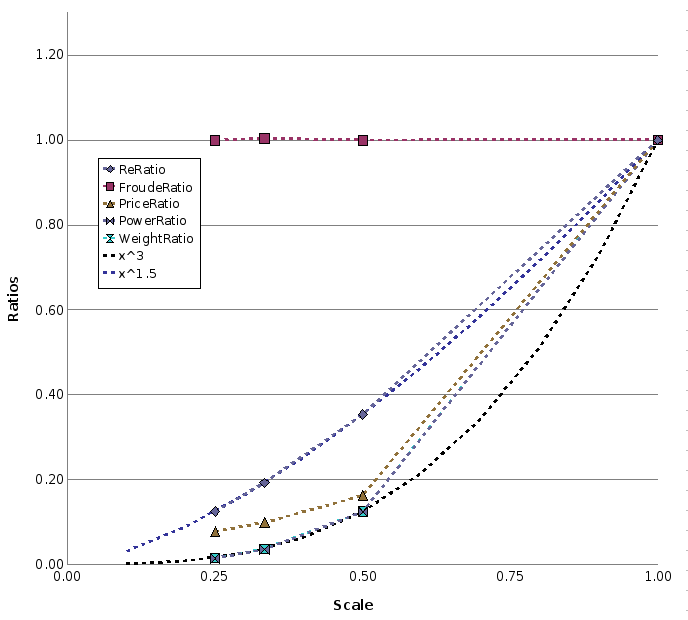
\includegraphics[width=140mm]{scale-graph.png}
\end{center}
\caption{Similitude Parameters versus Scale}
\label{fig:scales}
\end{figure}

\clearpage


\subsection{Autopilot and Sensors}
We are likely to fly the airplane with a remote controlled radio before moving to an autonomous vehicle. But even in the initial phases, having an autopilot which serves as an 'avionics' unit to log inputs and responses of the aircraft.\\

Since our goal is not particularly to develop a new autopilot, an off-the-shelf one would be preferable. We require a board that has enough PPM channels to command at least 8 servos and one Electronic-Speed-Controller, 3 serial ports (radio, GPS and IMU) and 5 to 8 A2D converters for the alpha-beta veins, pressure sensors, etc. Moreover, we would like to have fairly decent onboard computing power in the event we decide to use more advanced control algorithms or carry scientific payload. Unfortunately, most commercially available autopilots are closed-source and tend to be cost-prohibitive, which forces us to turn to the DIY scene. However, even the most mature DIY systems have limited processing power, serial and I/O ports.\\

For these reasons, we are considering to use the open-source \textit{Paparazzi} software in conjunction with a \textit{Roboard} hardware. We chose this architecture because the \textit{Roboard} hardware satisfies our requirements. A similar approach has been carried-out by other groups, and the \textit{Paparazzi} has a good track record of being used on different hardware architectures (ranging from Gumstix to x86 computers\footnote{A recent effort by students from Rutgers University has successfully ported the paparazzi to a beagleboard running linux http://moreproductive.org/autopilot/})\\

The reason we want to use the \textit{Paparazzi} is that after having worked with it for 6 months, we think that some of its functionalities such as in-flight tuning make flight-testing easier. Moreover, its support for both state-machine, 6DOF and HITL simulations help reduce development and testing time. The point is that while we could develop our own autopilot from scratch, we can avoid 'yet-another-autopilot' by leveraging the \textit{Roboard} and \textit{Paparazzi} capabilities and online communities.\\

\begin{figure}[h]
\begin{center}

\includegraphics[width = 30mm] {paparazzi.png}
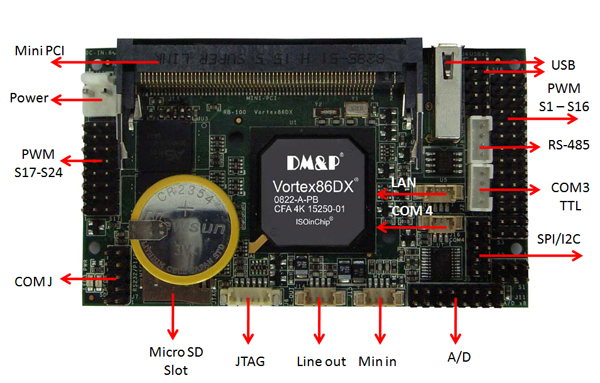
\includegraphics[width = 40mm] {Roboard.png}
\caption{Paparazzi Software and Roboard Hardware}
\end{center}
\end{figure}

\newpage
\subsection{Issues with small Reynolds numbers}
A 1/4 scale has the advantage of being roughly the size of most RC models, which means that flying it would be relatively easy. The problem however, is that at this scale Reynold numbers are so small that the airfoil characteristics are likely to suffer, especially at high lift-coefficients. In order to analyze the effect of this, we have used Xfoil to generate section data at different Reynolds numbers. The analysis is viscous and assumes a trip location at 20\% and N=13. We then used the results with a vortex-lattice code (XFLR5, figure \ref{fig:xflr3D} is a sample view of the 3D geometry. Cp distribution obtained from 3D panel code, but actual analysis uses VLM method) to generate angle-of-attack sweeps for the different scales and masses. The lift was constrained to match the weight so that different velocities and Reynolds numbers are used. The curves are truncated after one of the wing's sections stalls since the data can no longer be interpolated. \\

The results of using the same 17\% thick sections at different scales are shown in the first 4 plots of figure \ref{fig:tc17} (wing is at an incidence of $10^o$). We notice that the full-scale achieves a maximum ${C_L}$ of 1.3, while the 1/2 reaches ${C_L}_{max}\approx1.2$ and the 1/3 and 1/4 are way past stall by 0.9. Moreover, for the 1/3 and 1/4 scale there is a sharp decrease of the lift-to-drag ratio ${C_L}/{C_D}$ around ${C_L}=0.7$ (1 for the 1/2) indicating that portions of the wing have already started to stall. This is clearly unacceptable since we expect to cruise at ${C_L}=0.7$ (optimal L/D)\\

In order to fix this, we have decided to reduce the thickness to chord ratio of the airfoil sections while retaining the same camber line. This helps the flow to remain attached at higher lift coefficients despite the reduced Reynolds number. We first consider 13\% thick sections for all the scales, and the results are shown in the last 4 plots of figure \ref{fig:tc17}. This alone increases the ${C_L}_{max}$ to 1.2 for most of the scales, but we notice that the inboard sections of the 1/3 scale are stalled by the point they reach ${C_L}=0.9$ and at ${C_L}=0.8$ for the 1/4 (see appendix \ref{app:stalled})\\

Encouraged by the positive effect of decreasing the t/c, we further reduce it to 10\% to see if we can improve the curves. The results are in figure \ref{fig:tc10}. Clearly the maximum $C_L$ is improved for the 1/3 and 1/4 scales, but oddly enough this actually causes the 1/2 scale to stall at a smaller lift coefficient. Moreover, we notice that the shape of the L/D curve is significantly different now. This leads us to select the 13\% thick sections for the 1/2 scale and the 10\% sections for the 1/3 and 1/4 scale. It's worth mentioning that we also tried an even thinner section (7\%) for the 1/3 and 1/4 scale, but it did not improve the results. We believe that this is due to the 2D analysis in Xfoil having difficulty to find solutions for the thinner sections, maybe due to the fact that we use the same paneling as for the thick sections?. 

\enlargethispage{3\baselineskip}

\begin{landscape}
	\begin{figure}
	\begin{center}
	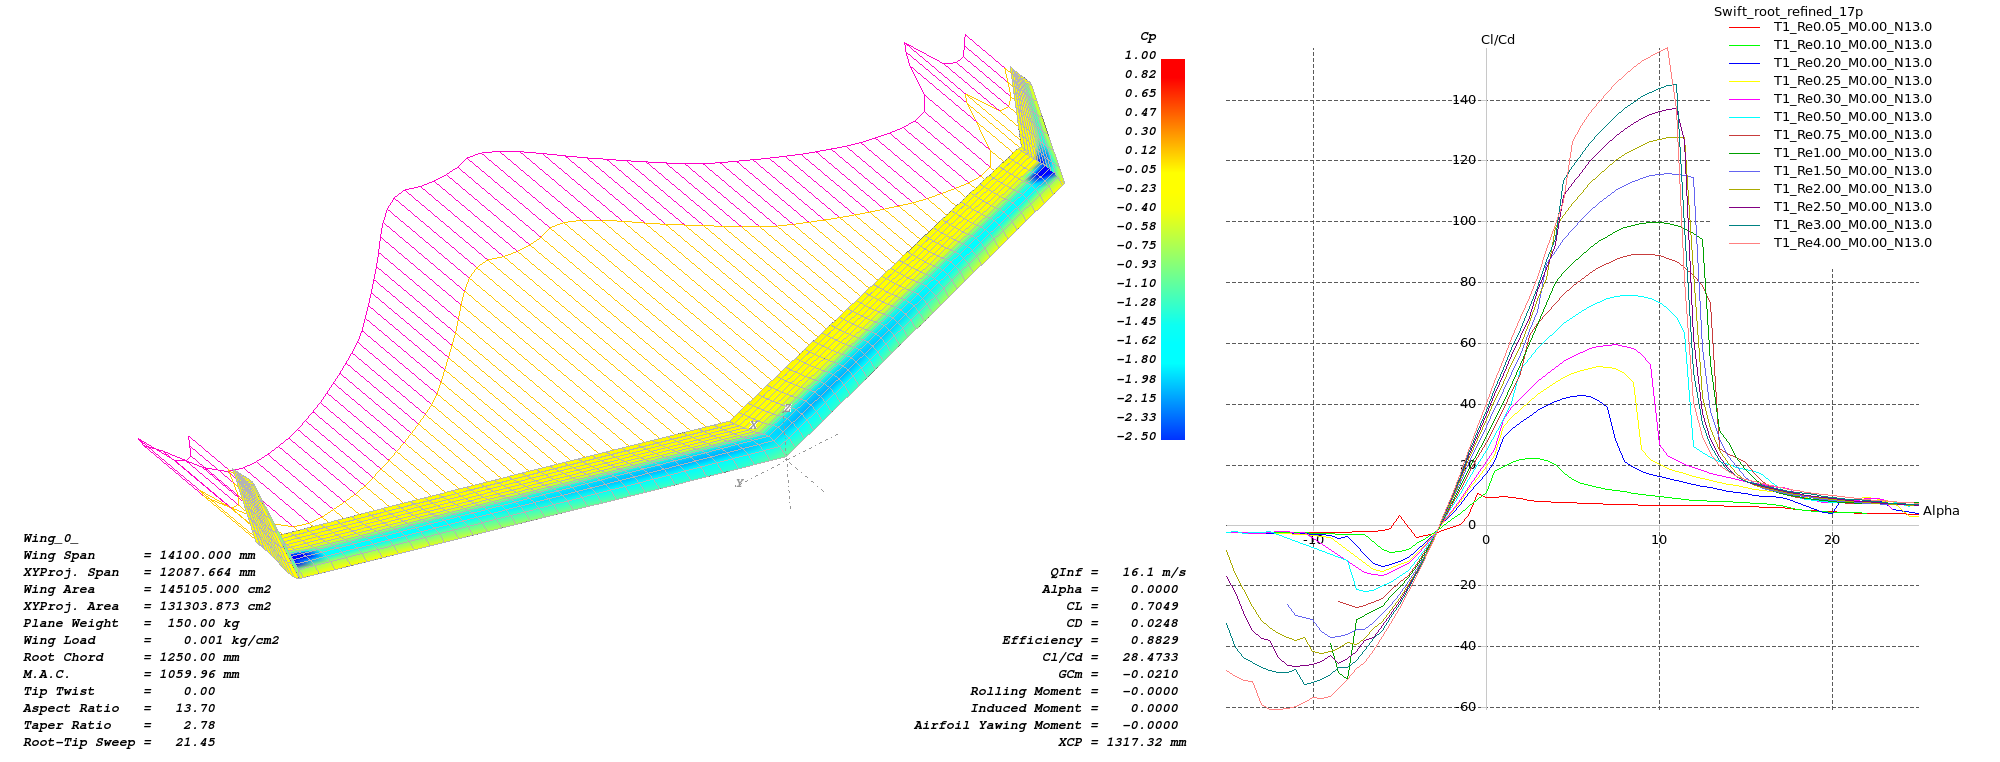
\includegraphics[width=220mm]{XFLR_3Dviews.png}
	\end{center}
	\caption{3D Geometry and $\frac{CL}{{C_D}}$ for typical section at different Re numbers}
	\label{fig:xflr3D}
	\end{figure}
\end{landscape}

\begin{figure}[h]
\begin{center}
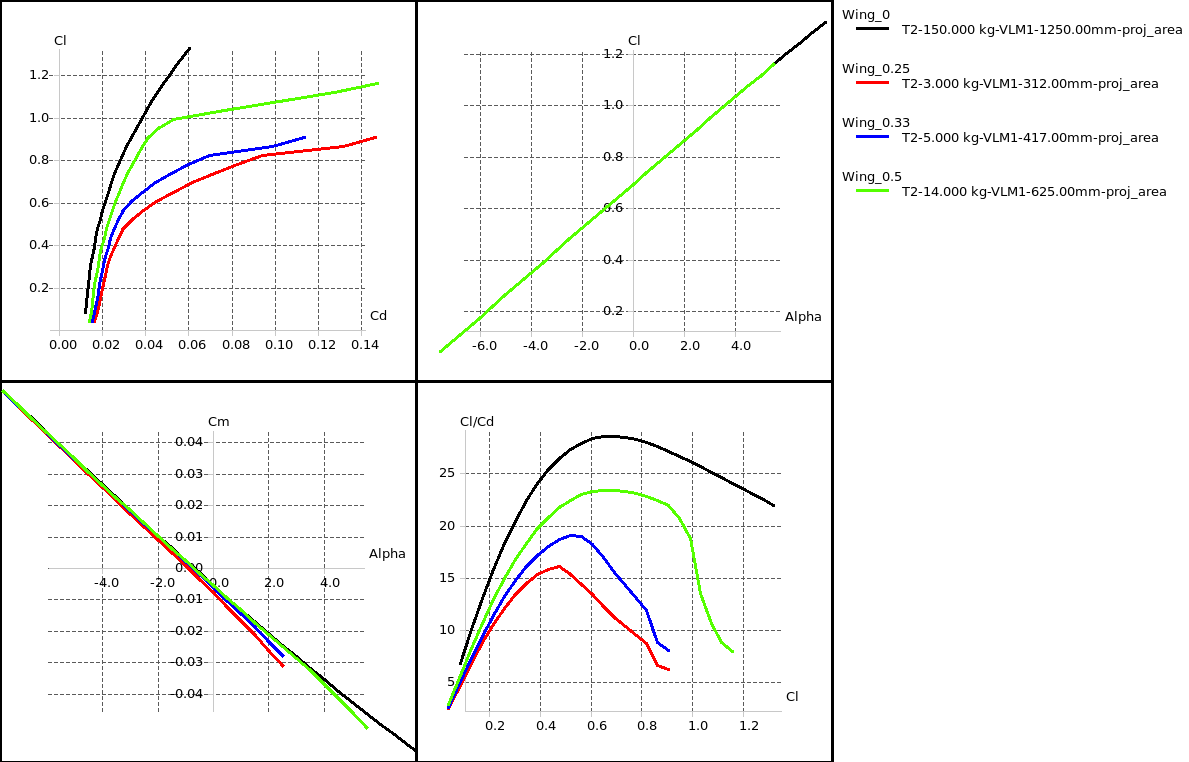
\includegraphics[width=120mm]{scale_original_airfoil_17.png}
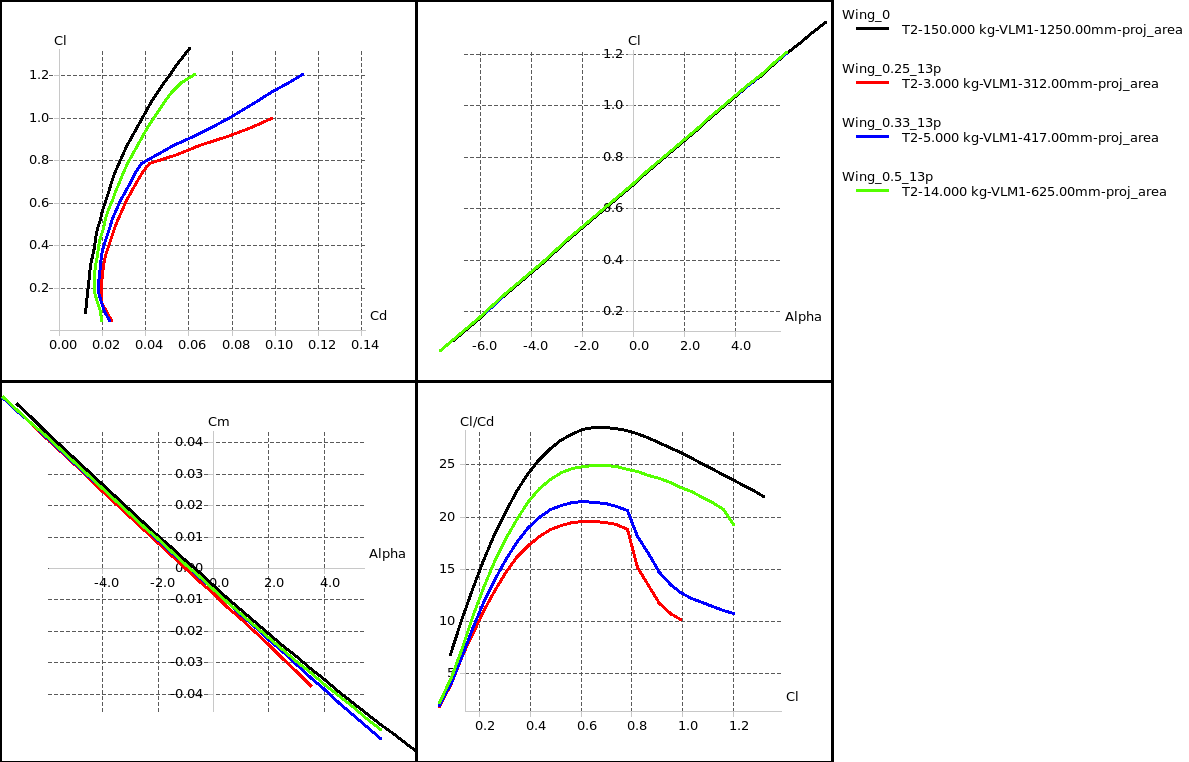
\includegraphics[width=120mm]{scale_tc_13.png}
\caption{17\% thick Airfoils for all scales versus 13\% thick Airfoils}
\label{fig:tc17}
\end{center}
\end{figure}

\begin{figure}[h]
\begin{center}
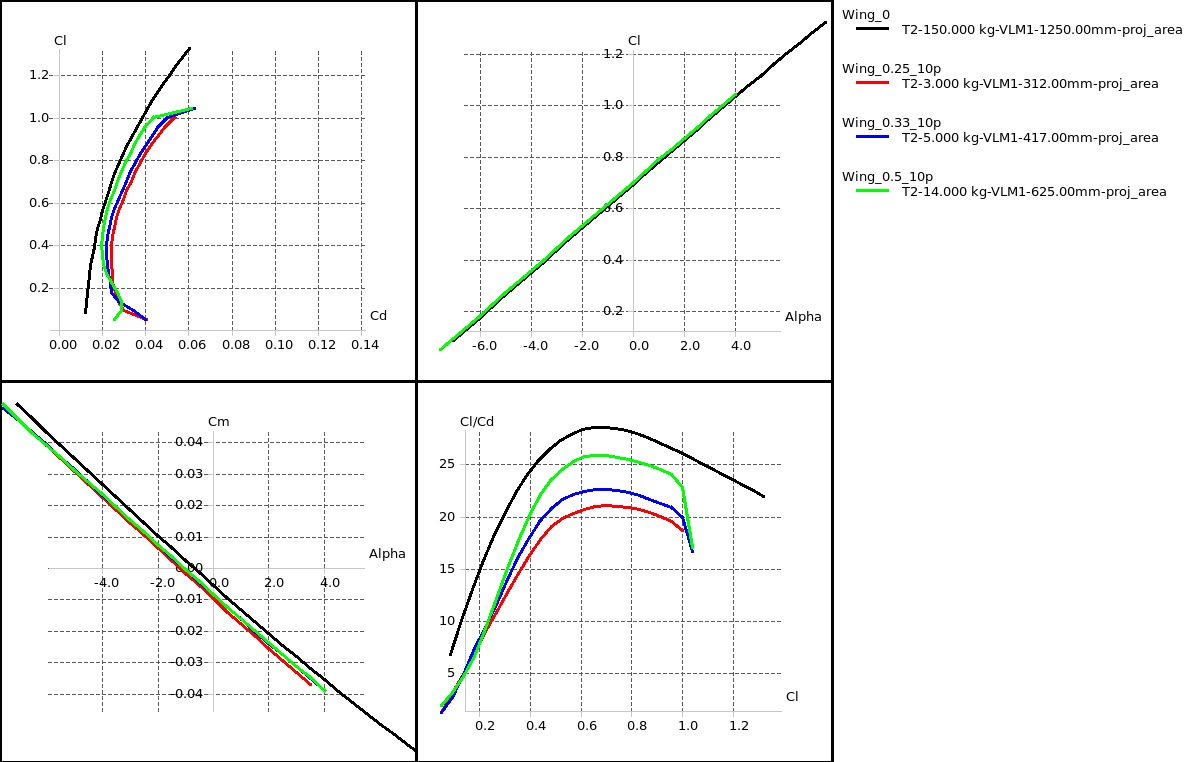
\includegraphics[width=120mm]{scale_tc_10.png}
\caption{10\% thick Airfoils for all scales}
\label{fig:tc10}
\end{center}
\end{figure}

\begin{figure}[h]
\begin{center}
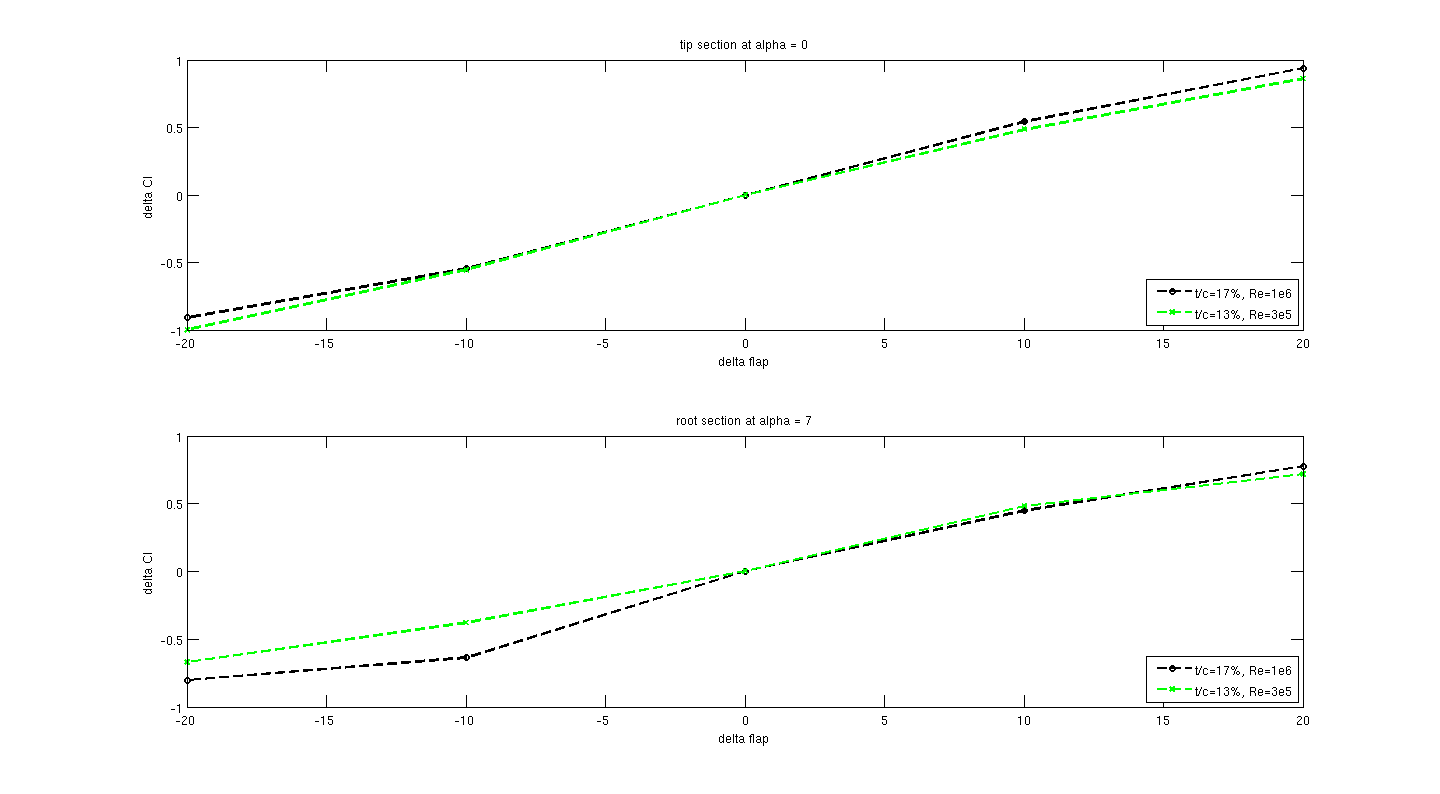
\includegraphics[width=140mm]{flap_effectiveness.png}
\caption{$\Delta CL_{\delta_{flap}}$ for 2D sections at $\alpha=0^o$ and  $\alpha=7^o$}
\label{fig:clflap}
\end{center}
\end{figure}
\clearpage


In all cases, the pitching moment coefficient ${C_m}$ and pitching moment derivative \footnote{CG position relative to the leading edge is at the same fraction of the MAC for all scales} ${C_m}_{\alpha}$ are hardly changed as predicted by thin airfoil theory \footnote{Small changes in Cm are due to difference in Boundary Layer thickness at different Re}. It's worth pointing out that the drag coefficient even for the 1/2 scale model is higher since airfoils have generally lower L/D at lower Reynolds numbers.\\

The next thing we looked at is how the Reynolds number and change in thickness would affect the effectiveness of the flaps. Figure \ref{fig:clflap} shows $\Delta CL_{\delta_{flap}}$ the change in lift coefficient caused by a flap deflection (flap down is +ve) at different Reynolds numbers and angles of attack. At 0 angle of attack, which is approximatively the AoA at the tip sections at cruise (remember the wing is at an incident of $10^o$ and the tips have a $10^o$ washout), there is very little difference between the 17\% and 13\% thick sections despite the fact that they operate at different Reynolds numbers. For $\alpha=7^o$ which is approximatively the AoA for the root sections at cruise (again wing at $10^o$ but there is about $-3^o$ of induced angle), there's little difference for downward flap deflection, but there seems to be a difference for negative flap deflections. Considering that the inboard flaps on the Swift are used mostly in the downward direction in order to change the $Cm_0$, we believe that the difference at the higher AoA for upward flap deflections should not be a major issue. To confirm this, we analyze the entire wing for the different scales with the inboard flaps deflected 10 and 20 degrees in the same direction (figure \ref{fig:tcflaps}), and with the outboard flaps (ailerons) deflected 10 and 20 in opposite directions (figure \ref{fig:tcailerons}).\\

First of all we notice again that the scale models are not able to achieve the same $CL_{max}$, but the 1/2 scale comes close to doing so. While the $\Delta {C_m}_{\delta_{flap}}$ show some relatively small differences, we notice that for all cases $\Delta {C_L}_{\delta_{flap}}$ is practically the same. This seems to indicate that that the effectiveness of the control surfaces would not suffer as far as flaps are concerned. Looking at figure \ref{fig:tcailerons}, we can see that for the case of ailerons the rolling moment is unchanged as well, but the (adverse) yawing moment due to the differential drag is definitely different. That being said, its absolute value is pretty small so even if there are differences we don't expect them to significantly influence the flight characteristics. A more worrying point is that it seems like there were issues with the analysis converging at higher angles-of-attack. However, this seems to be caused by a discontinuity at the intersection with the winglets where the software has difficulty properly interpolating the section geometry for an with a flap deflection.\\

Based on this analysis, a 10\% thick section for the 1/4 model and a 13\% thick section for the 1/3 and 1/2 models would mitigate some of the low Reynolds numbers issues, but it seems like only the 1/2 scale model is able to capture most of the flight envelope.


\begin{figure}[htbp]
\begin{center}
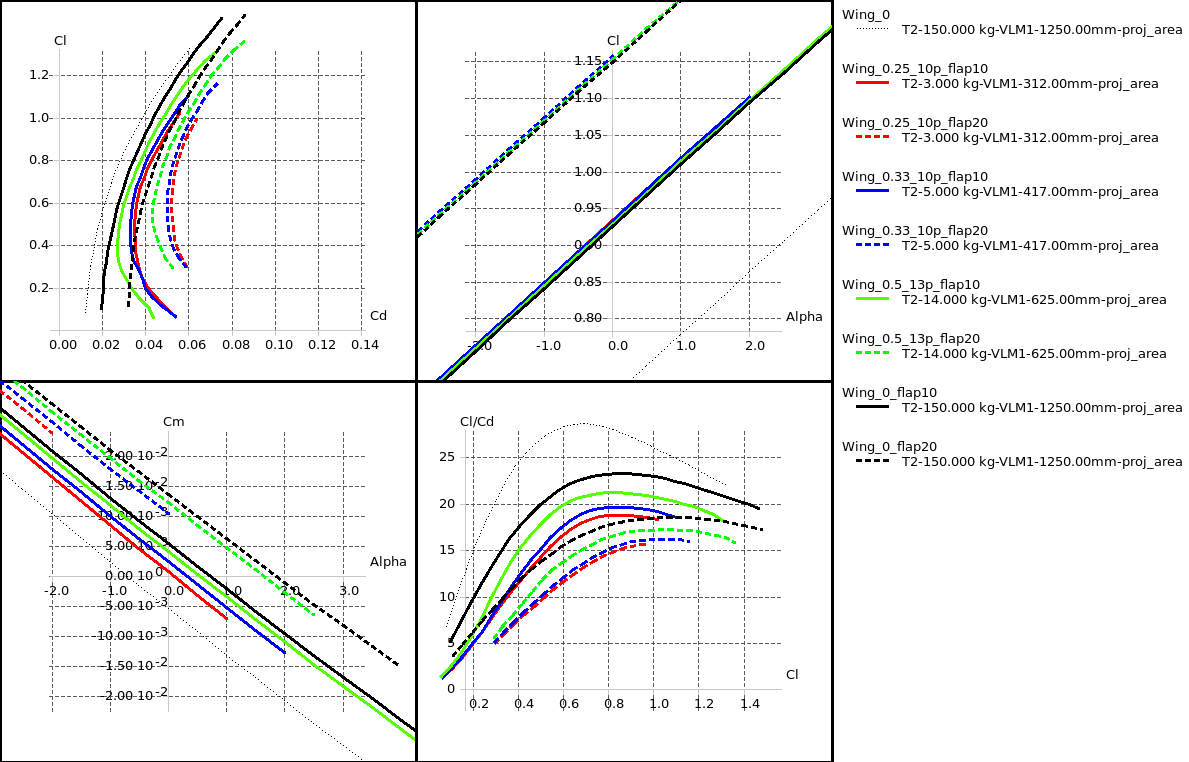
\includegraphics[width=120mm]{scale_tc_flaps.png}
\caption{Wing analysis with 10 and 20 degrees flaps}
\label{fig:tcflaps}
\end{center}
\end{figure}
\begin{figure}[htb]
\begin{center}
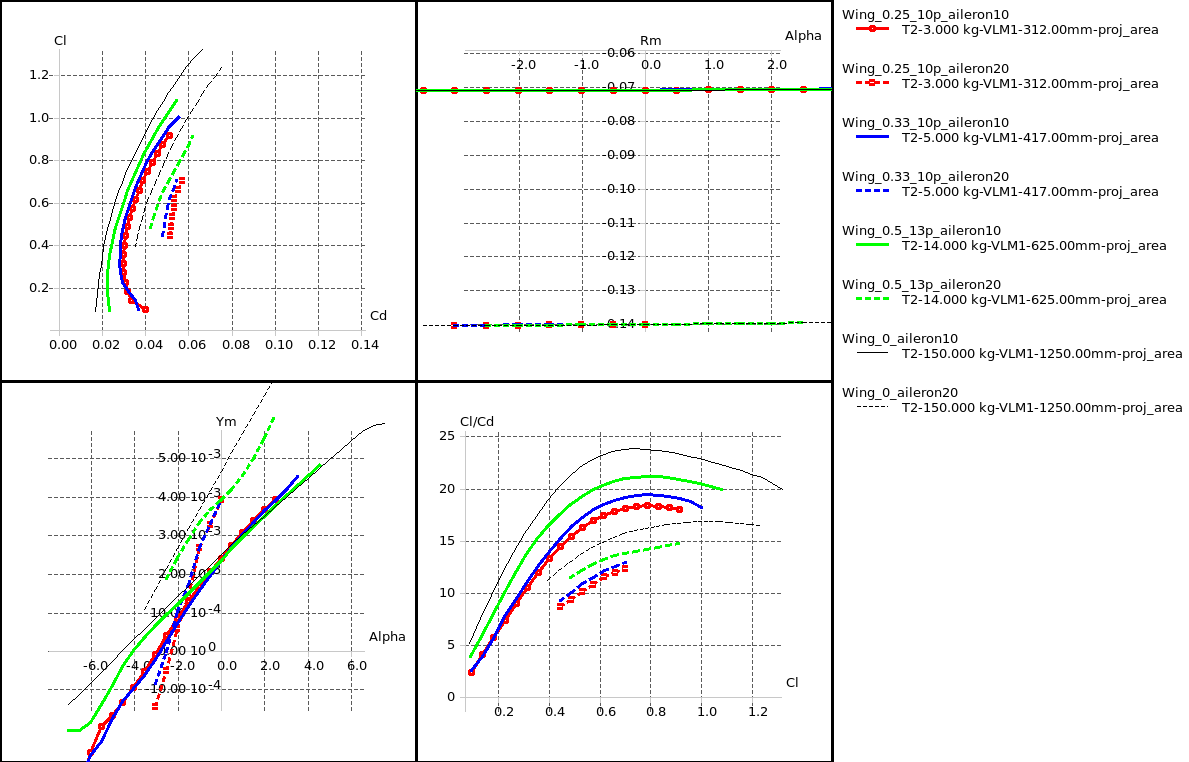
\includegraphics[width=120mm]{scale_tc_ailerons.png}
\caption{Wing analysis with 10 and 20 degrees ailerons}
\label{fig:tcailerons}
\end{center}
\end{figure}
\clearpage
\newpage

\subsection{Scaling and Measurements of Moments of Inertia}
One part that we have not addressed in the scaling is the difference in mass moments of inertia. While we don't expect them to have an effect on the stability derivatives and non-dimensional coefficients, they clearly will affect the longitudinal and lateral mode frequencies of the vehicle. So if the actual handling response is of interest, it probably is necessary to properly scale the moments of inertia in order to match the frequency response of the vehicle; on the other hand, if only the stability derivatives and non-dimensional coefficients are of interest, the scaling of the moments of inertia is of little importance as long as the vehicle remains stable.\\

That being said, sometimes a lot of effort goes into properly scaling the moments of inertia of a model. Per example, this has been done with the X-48B in order for the full-scale dynamic response to be accurately estimated from the sub-scale flight characteristics. An interesting question that can be investigated as part of this project is whether it's possible to synthesize an "co-pilot controller" that modifies the dynamics of the sub-scale model in order to match the frequency response of the full-scale vehicle. Moreover in order to estimate the aerodynamic coefficients from flight-tests, it is usually necessary to have good estimates of the mass and inertia properties of the airplane. Indeed, one of the conclusions of the preliminary flight test results of the X-48B is that there is a trade-off between estimating the kinematics and aerodynamics of the aircraft, and that \textit{"the parameter estimation [is] only as accurate as the aircraft inertia [estimates]}" \cite{X48B}.\\

While it is possible to measure inertias for a small sub-scale aircraft through a series of single degree-of-freedom oscillations, it can be a more challenging task for a larger aircraft where it's unsafe to hang the plane in all degrees, and therefore a meticulous component build-up is required. We believe that it might be possible to estimate moments of inertia from flight-tests as well. The idea would be to carry-out different flights where the weight and mass distribution of the airplane are carefully changed. Because the aerodynamic performance would remain unchanged (stability derivatives are only a function of the planform), it would be possible to estimate the inertia properties more accurately. We plan to investigate this technique on the small-scale plane and hopefully apply it to the full-scale one.\\
\enlargethispage{4 \baselineskip}

As far as the Swift is concerned, we currently only have rough estimates from CAD models of the wing geometry. We attempted to compare how the moments of inertia of the scaled models normalized by the Ixx values would compare to the full-scale. But because in our simplified weight estimation, the mass distribution ends up being roughly linear in the span position, the moments of inertia relative to each other end up being the same regardless of the scale. However, a more important non-dimensional measure of the moments of inertia is $I/(\rho c^5)$. 
\newpage

\begin{table}[h]
\begin{center}
\begin{tabular}{|l|c c c|}
\hline
Full scale & X & Y & Z \\
\hline
 & 517     &0.5	&-0.7 \\
 &	&17	&0.0 \\
 &	&	&533 \\
\hline
Half scale & & &\\
\hline		
 & 800	&0.80	&-1.1 \\
 &	&26	&0.00 \\
 &	&	&827 \\
\hline
Quarter scale & & &\\
\hline		
 & 846	&0.00	&-2.03 \\
 &	&26.33	&0.00 \\
 &	&	&873 \\
\hline
Third scale & & & \\
\hline		
 & 1088	&1.02	&-1.54 \\
 &	&35	&0.00 \\
 &	& 	&1123 \\
\hline
\end{tabular}
\caption{Moments of Inertia Scaling}
\label{tab:inertia}
\end{center}
\end{table}

Table \ref{tab:inertia} summarizes the moments of inertia of the wing as estimated by the CAD model normalized by the fifth power of the mean aerodynamic center. We notice that the 1/2 and 1/3 scale have similar normalized moments of inertia, but are different from those of the full scale. If the mass scales with $\lambda^3$, we would expect the inertia to scale with $\lambda^5$ and we should have constant normalized moments. However, in our estimates we only took into account the contribution of the wing, which in the case of the full scale is only 30\% of the vehicle weight, while it's more than 60\% for the half and third scale weights. This is mainly because the vehicles have vastly different endurances (i.e. one has relatively more batteries than the other). This means that while the mass of the entire vehicle appears to be proportional to $\lambda^3$, this is not the case for the wing, which explains the difference in the non-dimensional values.\\

At first these values are disconcerting since matching the moments of inertia is no longer just a question of adding ballast weight. But we have to keep in mind that we omitted the motor and batteries which account for more than half of the vehicle weight, so we actually underestimated the moments of inertia of the full-scale. However, since the batteries are relatively close to the center of gravity, we don't expect the moments of inertia to differ by more than a factor of 2 from our estimates. We are wary of making any conclusions just yet, but considering that the normalized values are within a factor of 2 of our current estimates, we should be able to properly match the inertias with a reasonable amount of ballast if necessary. Hopefully we will have more accurate estimates of the moments of inertia before we begin construction so that we may incorporate any necessary additional weight into the structure.


\newpage
\section{Conclusions}
The goal of this report was to identify potential research topics that can be pursued were we to build a sub-scale of the Swift. On the short term, a sub-scale vehicle would benefit NASA's full-scale UAV by providing a test-bed. On the long term, we would like to establish a theory and framework which would lead to a better understanding of effects of scaling on aerodynamic performance and dynamic response. There is of course also potential to use the vehicle by other Stanford affiliates as a testbed for new control algorithms, propeller noise characterization, electric propulsion system integration, etc. \\

Using a component buildup approach we estimated the total weight of the vehicle for different scales. We found that all three scales considered (1/2, 1/3 and 1/4) would be feasible using mostly off-the-shelf RC hobby parts. However, we identified that the smaller Reynolds numbers would be an issue, and investigated if changing the thickness-to-chord ratio of the airfoils while keeping the camber line fixed would mitigate some of the problems. We found that this works relatively well for the 1/2 scale case, where the stall-characteristics and control surface effectiveness do not suffer greatly. But while this also helps for the 1/3 and 1/4 scales, the flight-envelope is a little bit more restricted since the $CL_{max}$ is significantly lower than the full-scale. Finally, we made a small attempt to compare the non-dimensional moments of inertia, but did not come to any definite conclusion due to the fact that our estimates are not accurate enough.\\

Our analysis seems to indicate that a 1/4 scale would be the easiest to manufacture and operate, but will likely not allow us to match the full-scale performance. It also seems that there is little advantage in building a 1/3 scale over a 1/4 since it suffers from the same issues. The 1/2 scale on the other hand would allow us to match most of the flight-envelope, but is likely going to take longer to manufacture, and is more complicated in terms of operation.\\

In conclusion, building a 1/2 scale Swift would provide us with a vehicle that would be capable of matching the characteristics of the full-scale Swift while being about 10 times lighter, requiring 1/10th of the power and using affordable off-the-shelf parts. However, at that scale the airplane is likely going to have to be flown in restricted airspace. But at least it is likely to be classified under the Class-I low-risk category as opposed to medium or high risk like the the full-scale.




\subsection{Time-line and Future work}
\enlargethispage{3 \baselineskip}
This is a very rough time-line... \\
Design in Winter-Spring 2010: Settle on a scale, measure inertias on full-scale Swift, pick out components/sensors/etc, make drawings for subsystems, develop autopilot/FBW system, carry out more detailed analysis of the structure (especially if building 1/2 scale). Begin Construction in Summer 2010 ... Depending on scale, Initial flight-testing in Fall or Winter of next year.\\


\newpage
\appendix
\section{Weight, Power and Price Estimates}
\label{app:excel}
The results presented in section \ref{sec:initialsizing} were obtained from calculations using an Excel spreadsheet. In doing so, we used some assumptions to simplify the analysis. The spreadsheet is included with the report and has comments which summarize the content of this section.\\

Since the design of the airplane is technically already fixed, this greatly simplifies the weight estimation process. We break down the weight into four major subcomponents:

\subsection{Wing Weight}
\subsubsection{Foam core weight}
The weight of the foam core is computed using the wing volume which is obtained from a CAD model of the Swift. The density of the foam is assumed to vary between 21$kg/m^3$ and 37$kg/m^3$ depending on the scale of the model. That being said, for the 1/2 scale, we are likely not going to use a full foam core but rather a hollow one. The numbers reported here assume a full foam core, which means that are weight estimates are conservative.

\subsubsection{Skin Weight}
The skin weight is assumed to be proportional to the wetted area of the wing. Once again, this is obtained from a CAD model. The density of the skin is assumed to vary between 0.17$kg/m^2$ and 0.35$kg/m^2$ depending on the scale. In order to account for the weight of the resin, we researched the volume ratio of the fabric and using density of the resin estimated that the density of the matrix soaked in resin is a factor of 1.5 to 2.5 that of the fabric alone. We used an average of 2 in our calculation in the spreadsheet.

\subsubsection{Spar Weight}
We assume that we will be using carbon-fiber spar caps with a constant thickness. The design assumes an elliptical lift load which is integrated to find the maximum bending moment at each cross section along the span. We assume that the spars height is constrained by the width of the airfoil sections, while their width is a fixed percentage (5\%) of the root section chord. The required thickness to carry the bending load is then computed, and the entire volume is integrated to obtain the total mass of the spar. For simplicity, we precompute the percentage of the spar weight for a range of vehicle weights and use that inside the spreadsheet. The matlab routine used for this is included in appendix\ref{app:sparsizing}. 

\subsection{Fuselage Weight}
The fuselage is assumed to be constructed using the same material for the wing skin. The surface area of the fuselage is obtained from the CAD model and is approximatively 1/4th of the wing wetted area.

\subsection{Propulsion System Weight}
\subsubsection{Power Estimation}
In order to estimate the weight of the propulsion system, we need to first estimate the power required by the model plane. We begin by assuming a cruise lift coefficient and a lift-to-drag ratio (this could be estimated from a quadratic drag equation but we would have to assume a zero-lift drag coefficient instead). We also assume a propeller and propulsion efficiencies. We can use $$P_{cruise,req} = D*V_{cruise}/\eta = \frac{W\ V}{\eta \frac{L}{D}}$$ to estimate the required cruise power. However, we need to be able to achieve a minimum climb rate. So we use instead $P_{req} = T*V_{cruise}/\eta$ where T can be obtained from $(T-D)=\gamma*W$ with $\gamma$ being the climb path angle. Using these relations we find that $$P_{climb,req} = \frac{W\ V}{\eta \frac{L}{D}}(1+\gamma \frac{L}{D})$$
The spreadsheet takes a climb rate h as an input and computes $\gamma=h/V$. We estimated the climb rate of the full scale to be used $h=4m/s\approx800ft/min$ and used that in our calculations.

\subsubsection{Motor and actuator Weight}
Given the required power from the motor, we can use statistical methods to estimate the weight of the motor. We rely on the data given in the AxiMotors catalog to come up with simple fits. We were conservative in these estimates in order to allow for extra weight due to wires, ESC and propeller. As for the actuators, we were unable to find a simple relation between the torque rating and weight. So instead we assume a fixed weight per actuator with different values for each scale.

\subsubsection{Battery Weight}
The battery weight is computed by determining the required energy to achieve a desired endurance. The endurance can be set in the sheet and is assumed to be 20 minutes, with 30\% of it spent in climb and the rest in cruise. The battery capacity in mAh is then computed from the voltage (i.e. number of cells). Given the required capacity we can compute the weight by assuming an energy density which is fairly constant over a large range for Lithium Polymer batteries. 


\subsection{Avionics Weight}
We assume this to be a fixed weight which includes the autopilot board, sensors and a 2000mAh LiPo for power.


\subsection{Weight Iteration}
The motor weight estimation relies on the required power, which in turn is a function of the total weight. However, we initially don't know the total weight since we only estimate the structural weight. So we need to iterate until we converge to a total weight which accounts for the structural weight and propulsion weight. The same process needs to be carried out for the weight of the spars.

\subsection{Price Estimates}
Most of the price estimates are statistical fits to values quoted by online suppliers. Whenever possible an explanation or link is given in the spreadsheet. It's worth noting that the cost does not include 'tooling' cost as we assume it will be available at the lab.


\newpage	
\section{Stalled Inboard Sections}
\label{app:stalled}
In the analysis due to changes in Reynolds Numbers we have compared maximum lift coefficients and lift-to-drag ratios for the entire wing at different scales. We made the claim that although in some cases the entire wing is able to reach a high-lift coefficient, the sharp decrease of $C_L/C_D$ at lower values of $C_L$ indicate that the wing was partially stalled. The following figure which shows the span-wise distribution of the local drag coefficient $C_d$ of the three different scales at a fixed AoA and $C_L=0.8$. It's normal that $C_d$ increases as we approach the wing root since the local lift coefficient $C_l$ is higher due to the washout (the discontinuous at the tip are due to the winglets). However, it is clear that in the case of the 1/4 scale, there is an abrupt two fold increase in $C_d$, indicating that the inboard sections have stalled. We notice the same thing with the 1/3 scale, but not with the 1/2 scale.

\begin{figure}[h]
\begin{center}
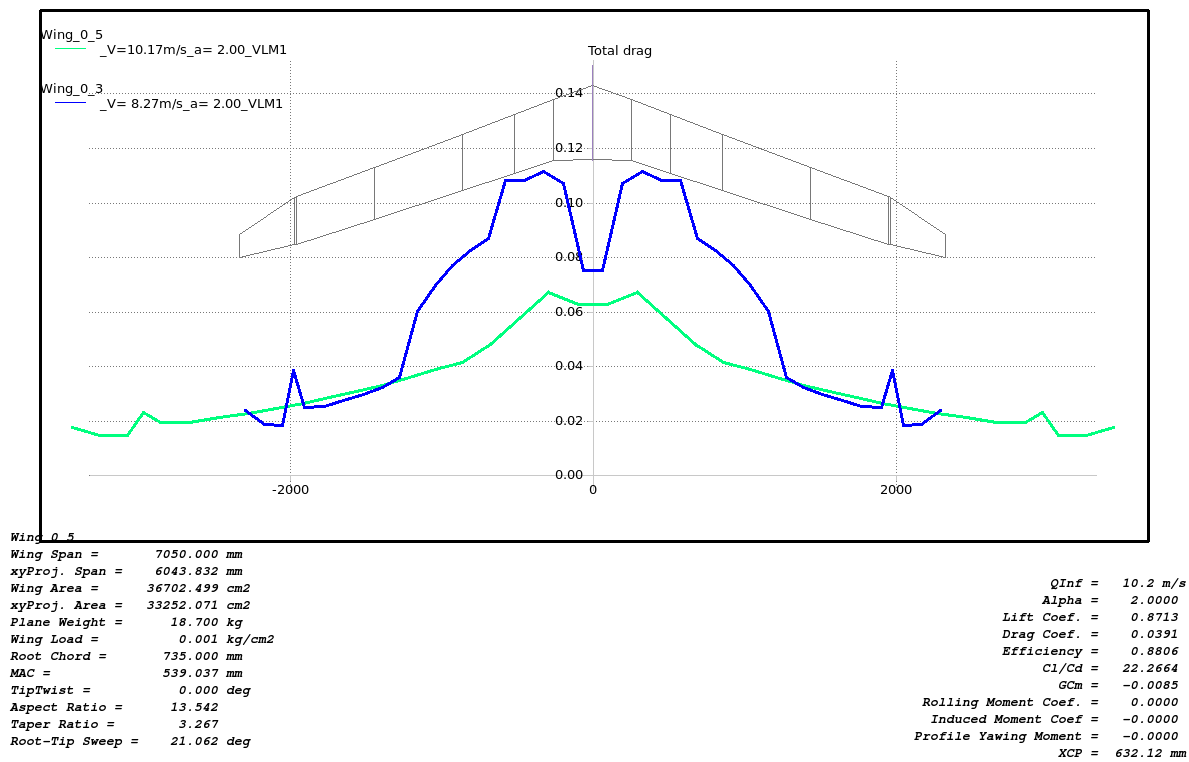
\includegraphics[width=120mm]{XFLR_spandrag_stall.png}
\end{center}
\caption{Spanwise distribution of the local drag coefficient}
\label{fig:tcdrag}
\end{figure}

\clearpage

\newpage
\section{Matlab Routine for Spar Sizing}
\label{app:sparsizing}
\verbatimtabinput[8]{spar_sizing.m}

\newpage
\begin{thebibliography}{9}

\bibitem{Wolowicz}
   Wolowicz, C.H., Bowman, Jr., J.S., and Gilbert, W.P.,
   “Similitude Requirements and Scaling Relationships as Applied to Model Testing”, 
   NASA TP-1435, 1979.

\bibitem{Airstar}
	Thomas L. Jordan, et Al.,
	"AirSTAR: A UAV Platform for Flight Dynamics and Control System Testing"
	NASA Langley Research Center, Hampton, VA 23681

\bibitem{X48B}
	Brian R Taylor,
	X-48B Preliminary Flight Test Results.
	Fundamentals Aeronautics Program, Subsonic Fixed Wing Project.
	2009 Annual Meeting


\end{thebibliography}


\end{document}
